%xelatex
\documentclass{article}
\usepackage[margin=0.6in]{geometry}
\usepackage{xltxtra}
\usepackage{xgreek}
\usepackage{listings}
\setmainfont[Mapping=tex-text]{Kerkis}
\usepackage[colorlinks=true,linkcolor=black,urlcolor=blue]{hyperref}
\title{Παράλληλη επεξεργασία}
\author{Μπαντολας Πέτρος 5028\\Σειμένης Σπύρος 5070\\Καλλιβωκάς Δημήτριος 4993}

\begin{document}
\maketitle
\section{Ανάλυση σειριακής έκδοσης}
- ΑΝΑΛΥΣΗ ΤΟΥ ΚΩΔΙΚΑ ΜΕ ΧΡΗΣΗ SCALASCA\\
- SCREENSHOT ΑΠΟ SCALASCA
- ..

\section{Παραλληλοποίηση}
\subsection{Με χρήση OpenMP}
Σύμφωνα με την προηγούμενη ανάλυση, τα σημεία όπου χρειάζεται χρονοβελτίωση είναι κυρίως οι κλήσεις της \texttt{dist} μέσα στις συναρτήσεις \texttt{pgain} και \texttt{pspeedy}.

Δύο είναι τα σημεία μέσα στην \texttt{pgain} όπου καλείται σε βρόχο \texttt{for} η \texttt{dist}. Εισάγοντας εκεί εντολές \texttt{OpenMP} μειώνεται αρκετά ο χρόνος εκτέλεσης.

Ακόμη, στη συνάρτηση \texttt{pspeedy} καλείται σε ένθετο βρόχο η \texttt{dist}. Εισάγοντας σε αυτό το σημείο παραλληλοποίηση με \texttt{OpenMP} παρατηρείται μια μικρή βελτίωση στο χρόνο.

\begin{center}
\begin{tabular}{|r|c|l|}
    \hline
    Νήματα & Χρόνος Εκτέλεσης (-Ο0) & Χρόνος Εκτέλεσης (-Ο3) \\ \hline
    1 & 79.8 sec & 28.4 sec \\
    2 & 43.1 sec & 16.2 sec \\
    4 & 26.2 sec & 12.4 sec \\ \hline
\end{tabular}
\end{center}

\subsection{Με χρήση εντολών SIMD}
-ΑΙΤΙΟΛΟΓΗΣΗ ΒΕΛΤΙΣΤΟΠΟΙΗΣΗΣ
-ΜΕΤΡΗΣΕΙΣ






\end{document}



%\begin{center}
%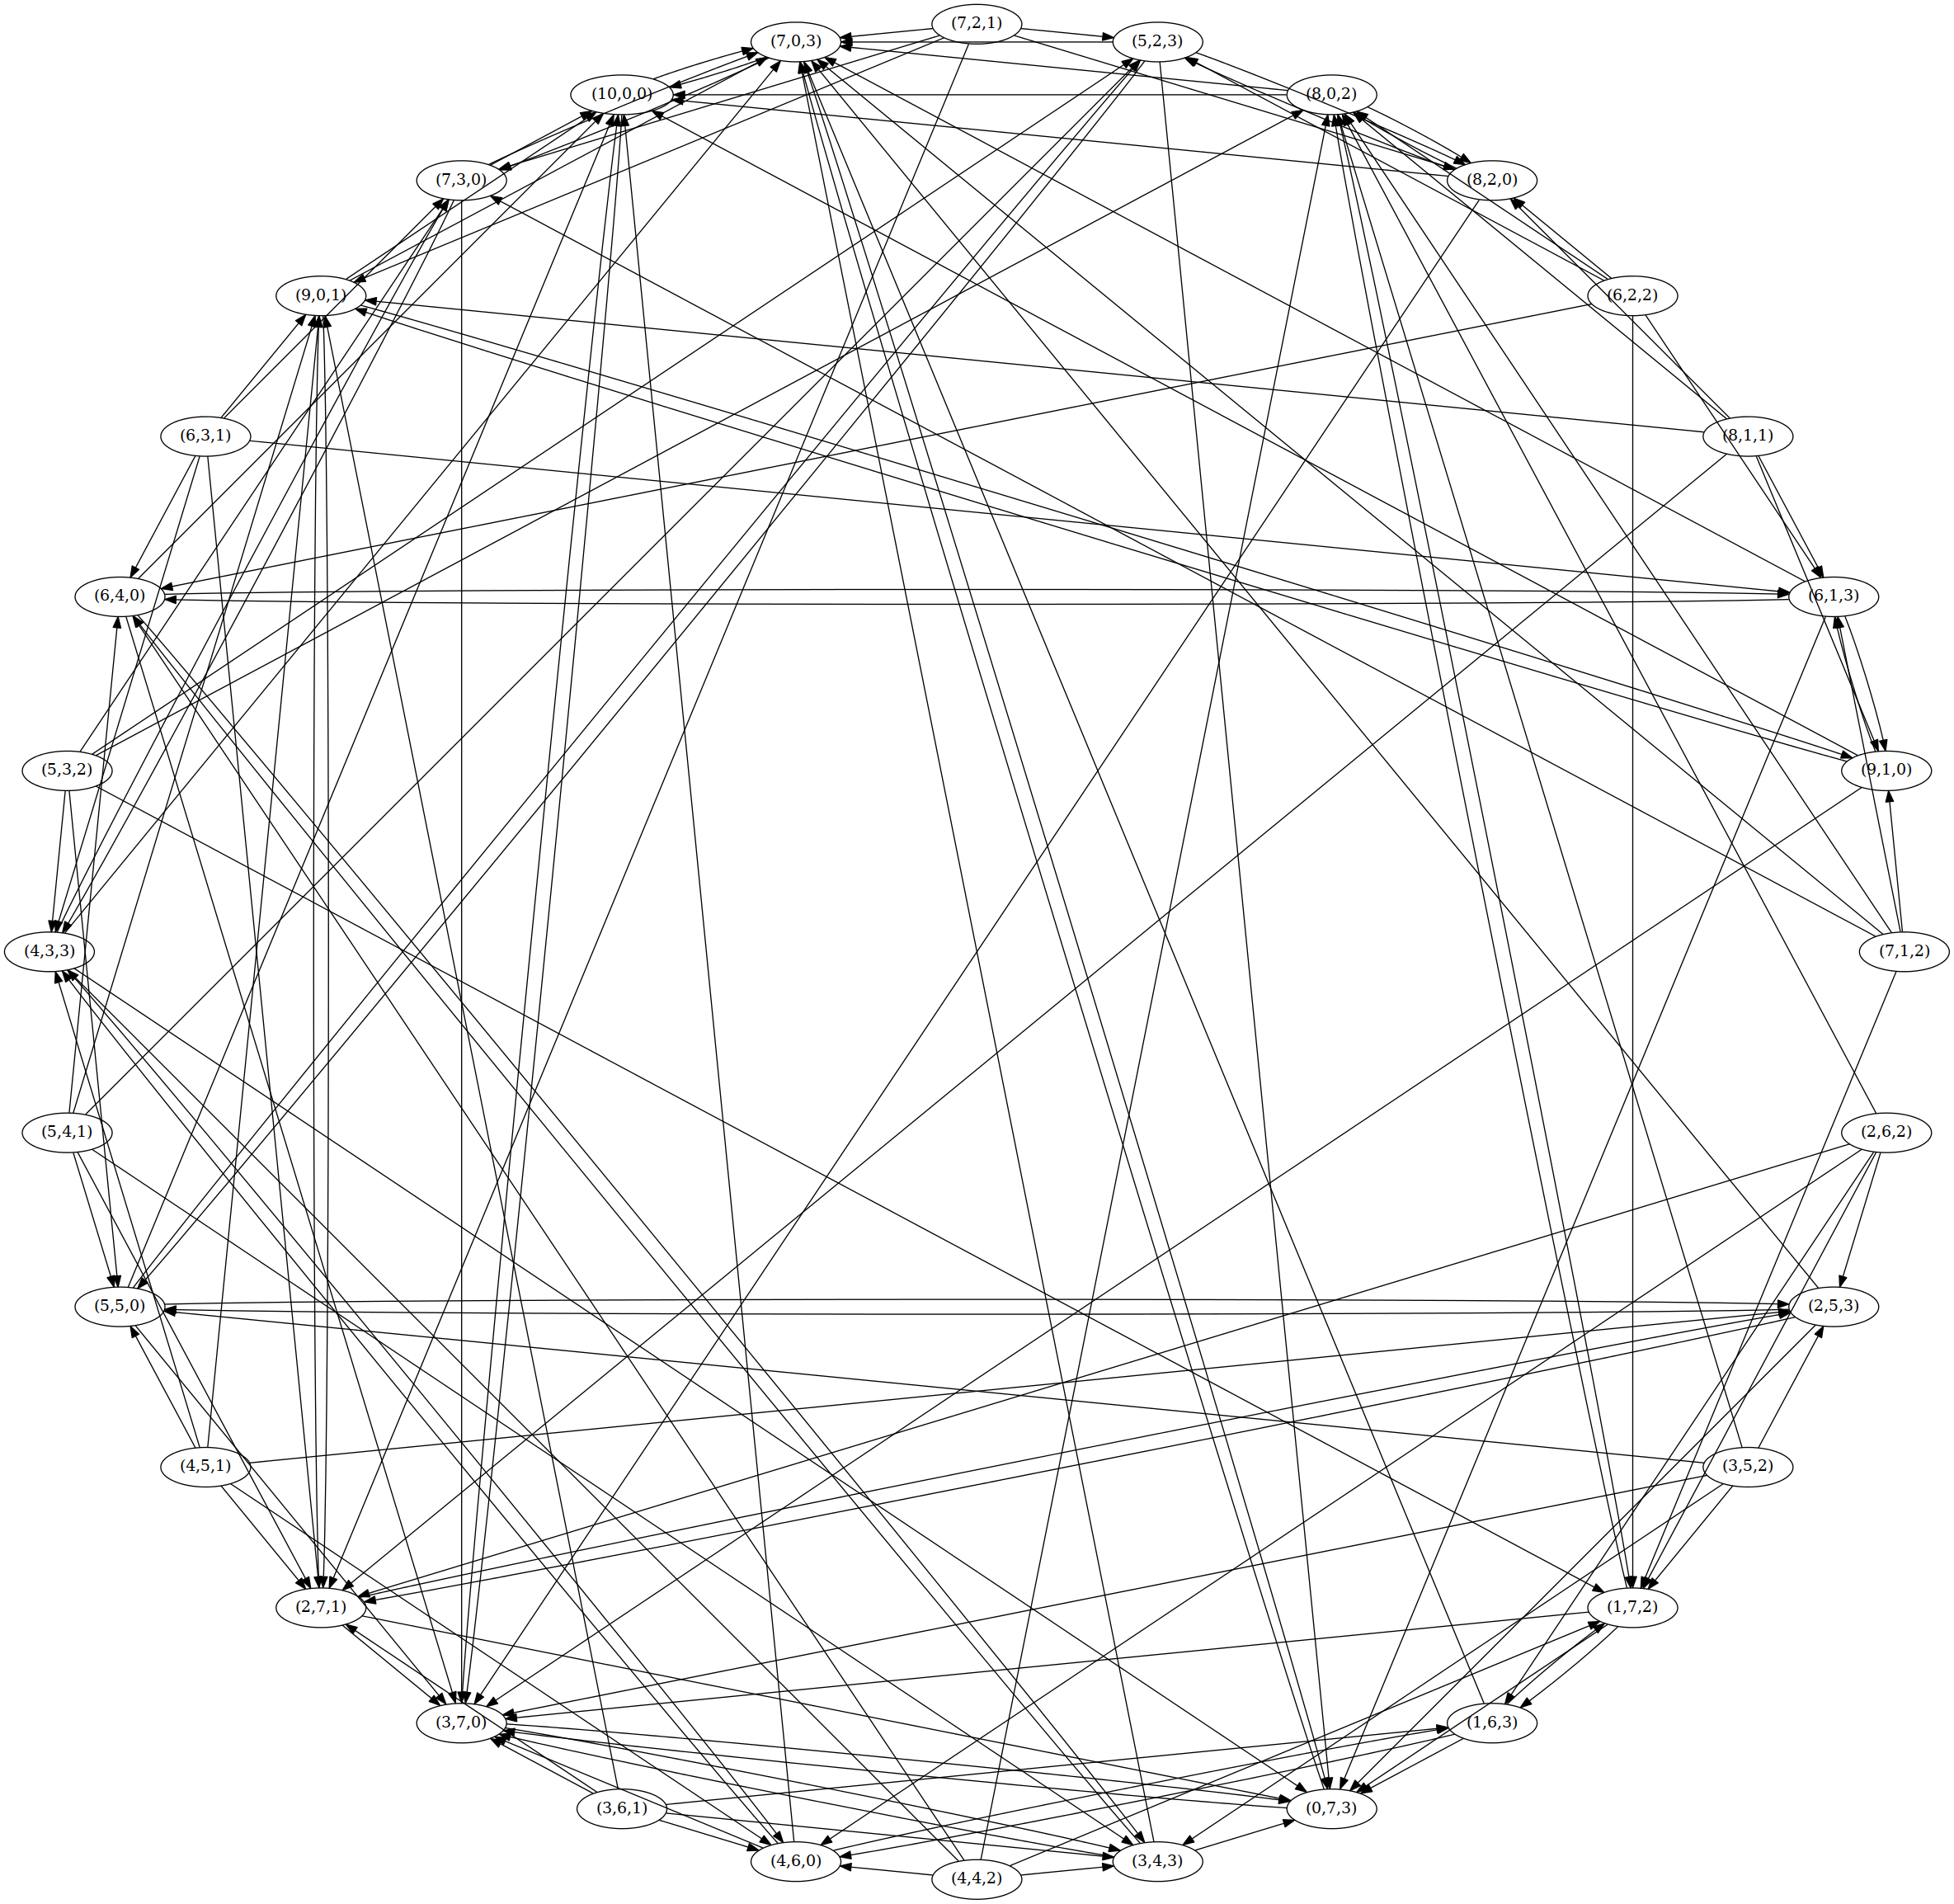
\includegraphics[scale=0.18]{../graph.png}
 % graph.png: 2369x2308 pixel, 300dpi, 20.06x19.54 cm, bb=0 0 569 554
%\end{center} 
